\Opensolutionfile{ans}[ans/ansCD2D1-5]

\begin{dang}{Đồ thị của đạo hàm}
\end{dang}
\paragraph{Các ví dụ}
\begin{vd}%[Dự án TLDH1-Nhóm Latex, Kiều Ngân]%[2D1B5-5]%Ví dụ 1.
	\immini{
	Cho hàm số $y=f(x)$. Hàm số $y=f'(x)$ có đồ thị như hình bên. Khẳng định nào sau đây là đúng?
	\choice
	{\True Đồ thị hàm số $y=f(x)$ có ba điểm cực trị}
	{Đồ thị hàm số $y=f(x)$ có hai điểm cực trị}
	{Đồ thị hàm số $y=f(x)$ có một điểm cực trị}
	{Đồ thị hàm số $y=f(x)$ không có điểm cực trị}
	}{
		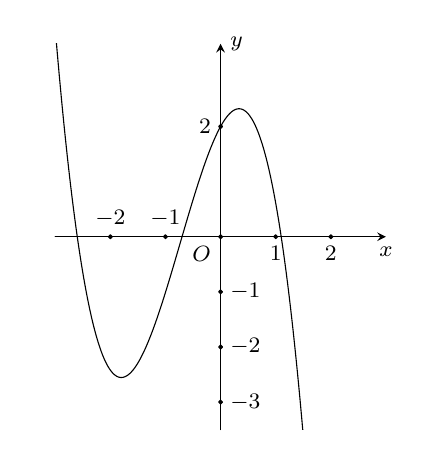
\begin{tikzpicture}[>=stealth,line join=round,line cap=round,font=\footnotesize,scale=0.7]
		\draw[->] (-3,0)--(3,0)node[below]{$x$};
		\draw[->] (0,-3.5)--(0,3.5)node[right]{$y$};
		\def\a{-1};
		\def\b{-2.2};
		\def\c{1.81};
		\def\d{2};
		\def\f(#1){\a*(#1)^3+\b*(#1)^2+\c*(#1)^1+\d};
		\clip (-3.5,-3.5)rectangle (3.5,3.5);		
		\draw[smooth,samples=300]
		plot[domain=-3:1.5](\x,{\f(\x)});
		\draw[fill=black] (0,0) circle (1pt) node[below left]{$O$};
		\draw[fill=black] (-2,0) circle (1pt) node[above]{$-2$};
		\draw[fill=black] (-1,0) circle (1pt) node[above]{$-1$};
		\draw[fill=black] (2,0) circle (1pt) node[below]{$2$};
		\draw[fill=black] (1,0) circle (1pt) node[below]{$1$};
		\draw[fill=black] (0,2) circle (1pt) node[left]{$2$};
		\draw[fill=black] (0,-1) circle (1pt) node[right]{$-1$};
		\draw[fill=black] (0,-2) circle (1pt) node[right]{$-2$};
		\draw[fill=black] (0,-3) circle (1pt) node[right]{$-3$};
		\end{tikzpicture}
	}
	\loigiai{
		Dựa vào đồ thị ta có $f'(x)$ cắt trục hoành tại ba điểm và đổi dấu $3$ lần, do đó đồ thị hàm số $y=f(x)$ có ba điểm cực trị.}
\end{vd}
\begin{vd}%[Dự án TLDH1-Nhóm Latex, Kiều Ngân]%[2D1B5-5]%Ví dụ 2.
	\immini{
		Hình bên là đồ thị của hàm số $y=f'(x)$. Hỏi hàm số $y=f(x)$ đồng biến trên khoảng nào dưới đây?
		\choice
		{$(1;2)$}
		{\True $(2;+\infty)$}
		{$(0;1)$ và $(2;+\infty)$}
		{$(0;1)$}
	}{
		\begin{tikzpicture}[>=stealth,line join=round,line cap=round,font=\footnotesize,scale=1.1]
		\draw[->] (-0.5,0)--(2.5,0)node[below]{$x$};
		\draw[->] (0,-1)--(0,1)node[right]{$y$};
		\def\a{1};
		\def\b{-4};
		\def\c{5};
		\def\d{-2};
		\def\f(#1){\a*(#1)^3+\b*(#1)^2+\c*(#1)^1+\d};
		\clip (-0.5,-1) rectangle (3,1);		
		\draw[smooth,samples=300]
		plot[domain=0.25:2.4](\x,{\f(\x)});
		\draw[fill=black] (0,0) circle (1pt) node[below left]{$O$};
		\draw[fill=black] (2,0) circle (1pt) node[below]{$2$};
		\draw[fill=black] (1,0) circle (1pt) node[below]{$1$};
		\end{tikzpicture}
	}
	
	\loigiai{
		Dựa vào đồ thị hàm số $y=f'(x)$ ta thấy $f'(x)>0,\forall x>2$.\\
		Vậy hàm số $y=f(x)$ đồng biến trên khoảng $(2;+\infty)$.}
\end{vd}
\begin{vd}%[Dự án TLDH1-Nhóm Latex, Kiều Ngân]%[2D1K5-5]%Ví dụ 3.
	\immini{
		Cho hàm số $f(x)$ xác định trên $\mathbb{R}$ và hàm số $y=f'(x)$ có đồ thị như hình vẽ. Xét hàm số $g(x)=f\left(x^2-2\right)$. Mệnh đề nào sau đây đúng?
		\choice
		{Hàm số $g(x)$ đồng biến trên $\left(-\sqrt{5};\sqrt{5}\right)$}
		{Hàm số $g(x)$ nghịch biến trên $(-\infty;2)$}
		{Hàm số $g(x)$ nghịch biến trên $\left(-2;\sqrt{5}\right)$}
		{\True Hàm số $g(x)$ nghịch biến trên $\left(-\sqrt{5};-2\right)$}
	}{
		\begin{tikzpicture}[>=stealth,line join=round,line cap=round,font=\footnotesize,scale=1]
		\draw[->] (-0.5,0)--(4,0)node[below]{$x$};
		\draw[->] (0,-0.5)--(0,4.5)node[right]{$y$};
		\def\f(#1){-0.6*(#1-1)*(#1-2)*(#1-3)};
		\clip (-0.5,-1) rectangle (3.5,5);		
		\draw[smooth,samples=300]
		plot[domain=-0.1:3.25](\x,{\f(\x)});
		\draw[fill=black] (0,0) circle (1pt) node[below left]{$O$};
		\draw[fill=black] (2,0) circle (1pt) node[below]{$2$};
		\draw[fill=black] (1,0) circle (1pt) node[below]{$1$};
		\draw[fill=black] (3,0) circle (1pt) node[below]{$3$};
		\end{tikzpicture}
	}
	
	\loigiai{
		Ta có $g'(x)=2xf'\left(x^2-2\right)$.\\
		Bảng biến thiên của hàm số $y=f(x)$ như sau
		\begin{center}
			
\begin{tikzpicture}[>=stealth]
			\tkzTabInit[nocadre=false,lgt=1.2,espcl=2,deltacl=0.5]
			{$x$/.7 ,$f'(x)$/.7,$f(x)$/1.5}
			{$-\infty$, $1$, $2$, $3$, $+\infty$}
			\tkzTabLine{,+,$0$,-,$0$,+,$0$,-,}
			\tkzTabVar{-/, +/,-/, +/, -/}
			\end{tikzpicture}
		\end{center}
		Hàm số $g(x)$ nghịch biến nếu $g'(x)=2xf'\left(x^2-2\right)<0$
		\allowdisplaybreaks
		\begin{eqnarray*}
			&\Leftrightarrow&\hoac{&\heva{&x<0\\&f'\left(x^2-2\right)>0}\\&\heva{&x>0\\&f'\left(x^2-2\right)<0}}\Leftrightarrow\hoac{&\heva{&x<0\\&\hoac{&x^2-2<1\\&2<x^2-2<3}}\\&\heva{&x>0\\&\hoac{&1<x^2-2<2\\&x^2-2>3}}}\\
			&\Leftrightarrow&\hoac{&\heva{&x<0\\&\hoac{&-\sqrt{3}<x<\sqrt{3}\\&2<x<\sqrt{5}\\&-\sqrt{5}<x <-2}}\\&\heva{&x>0\\&\hoac{&-2<x <-\sqrt{3}\\&\sqrt{3}<x<2\\&x>\sqrt{5}\\&x <-\sqrt{5}}}}\Leftrightarrow\hoac{&x\in\left(-\sqrt{5};-2\right)\cup\left(-\sqrt{3};0\right)\\&x\in(\sqrt{3};2)\cup\left(\sqrt{5};+\infty\right).}
		\end{eqnarray*}
	}
\end{vd}
\begin{vd}%[Dự án TLDH1-Nhóm Latex, Kiều Ngân]%[2D1K5-5]%Ví dụ 4.
	Cho hàm số $y=f(x)$ có đạo hàm $f'(x)=x^2(x-9)(x-4)^2$. Xét hàm số \linebreak $y=g(x)=f(x^2)$ trên $\mathbb{R}$. Trong các phát biểu sau:\\
	I. Hàm số $y=g(x)$ đồng biến trên $(3;+\infty)$.\\
	II. Hàm số $y=g(x)$ nghịch biến trên $(-\infty;-3)$.\\
	III. Hàm số $y=g(x)$ có $5$ cực trị.\\
	IV. $\min\limits_{x\in\mathbb{R}} g(x)=f(9)$.\\
	Số phát biểu đúng là
	\choice
	{$1$}
	{$2$}
	{\True $3$}
	{$4$}
	\loigiai{
		Ta có $y'=g'(x) =2xf'(x^2) =2x^5(x^2-9)(x^2-4)^2$.\\
		$\left(x^2-4\right)^2\geq 0$ với mọi $x$, nên ta có thể xem như $g(x)$ có bảng biến thiên sau
		\begin{center}
			
\begin{tikzpicture}[>=stealth]
			\tkzTabInit[nocadre=false,lgt=1.2,espcl=2,deltacl=0.5]
			{$x$/.7 ,$g'(x)$/.7,$g(x)$/2}
			{$-\infty$, $-3$, $0$, $3$, $+\infty$}
			\tkzTabLine{,-,$0$,+,$0$,-,$0$,+,}
			\tkzTabVar{+/ $+\infty$, -/$f(9)$,+/$f(0)$, -/$f(9)$, +/$+\infty$}
			\end{tikzpicture}
		\end{center}
		Các khẳng định đúng là I, II và IV.}
\end{vd}
\begin{vd}%[Dự án TLDH1-Nhóm Latex, Kiều Ngân]%[2D1K5-5]%Ví dụ 5.
	\immini{
		Cho hàm số $f(x)$. Biết hàm số $y=f'(x)$ có đồ thị như hình bên. Trên đoạn $[-4;3]$, hàm số $g(x)=2f(x)+(1-x)^2$ đạt giá trị nhỏ nhất tại điểm
		\choice
		{$x_0=-4$}
		{\True $x_0=-1$}
		{$x_0=3$}
		{$x_0=-3$}
	}{
		\begin{tikzpicture}[>=stealth,line join=round,line cap=round,font=\footnotesize,scale=0.6]
		\draw[->] (-5,0)--(5,0)node[below]{$x$};
		\draw[->] (0,-3)--(0,6)node[right]{$y$};
		\def\f(#1){-0.1*(#1)^3-0.3*(#1)^2-0.4*(#1)^1+1.8};
		\def\g(#1){-0.175*(#1)^3+0.15*(#1)^2-0.075*(#1)^1+1.6};
		
		\clip (-5,-3) rectangle (5,6);		
		\draw[smooth,samples=300]
		plot[domain=-4.2:-1](\x,{\f(\x)});
		\draw[smooth,samples=300]
		plot[domain=-1:3.2](\x,{\g(\x)});
		\draw [dashed](-4,0)--(-4,5)--(0,5);
		\draw [dashed](-3,0)--(-3,3)--(0,3);
		\draw [dashed](-1,0)--(-1,2)--(0,2);
		\draw [dashed](3,0)--(3,-2)--(0,-2);
		\draw[fill=black] (0,0) circle (1pt) node[below right]{$O$};
		\draw[fill=black] (-4,0) circle (1pt) node[below]{$-4$};
		\draw[fill=black] (-3,0) circle (1pt) node[below]{$-3$};
		\draw[fill=black] (-1,0) circle (1pt) node[below]{$-1$};
		\draw[fill=black] (1,0) circle (1pt) node[below]{$1$};
		\draw[fill=black] (3,0) circle (1pt) node[above]{$3$};
		\draw[fill=black] (0,-2) circle (1pt) node[left]{$-2$};
		\draw[fill=black] (0,2) circle (1pt) node[right]{$2$};
		\draw[fill=black] (0,3) circle (1pt) node[right]{$3$};
		\draw[fill=black] (0,5) circle (1pt) node[right]{$5$};
		\draw[fill=black] (-4,5) circle (1pt);
		\draw[fill=black] (-3,3) circle (1pt);
		\draw[fill=black] (-1,2) circle (1pt);
		\draw[fill=black] (3,-2) circle (1pt);
		\end{tikzpicture}
	}
	
	\loigiai{
		\immini{
			Trên đoạn $[-4;3]$, ta có $g'(x)=2f'(x)-2(1-x)$.\\
			$g'(x)=0\Leftrightarrow f'(x)=1-x\Leftrightarrow\hoac{&x=-4\\&x=-1\\&x=3.}$\\
			Dựa vào đồ thị ta có bảng biến thiên của hàm số $g(x)$ như sau
			\begin{center}
				
\begin{tikzpicture}[>=stealth]
				\tkzTabInit[nocadre=false,lgt=1.2,espcl=2,deltacl=0.5]
				{$x$/.7 ,$g'(x)$/.7,$g(x)$/1.5}
				{$-4$, $-1$, $3$}
				\tkzTabLine{$0$,-,$0$,+,$0$}
				\tkzTabVar{+/,-/$g(-1)$,+/}
				\end{tikzpicture}
			\end{center}
			Suy ra hàm số $g(x)$ đạt giá trị nhỏ nhất tại điểm $x_0=-1$.
		}{
			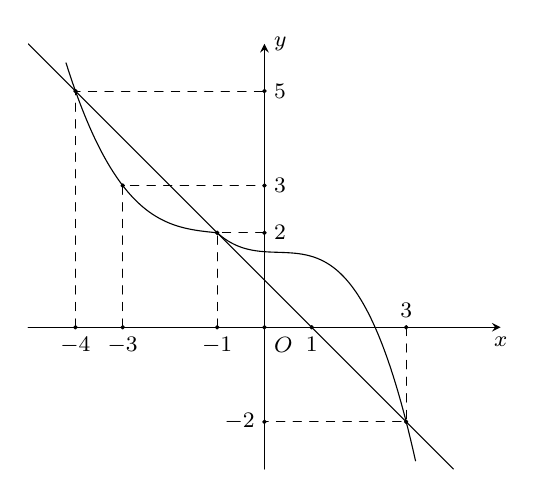
\begin{tikzpicture}[>=stealth,line join=round,line cap=round,font=\footnotesize,scale=0.6]
			\draw[->] (-5,0)--(5,0)node[below]{$x$};
			\draw[->] (0,-3)--(0,6)node[right]{$y$};
			\def\f(#1){-0.1*(#1)^3-0.3*(#1)^2-0.4*(#1)^1+1.8};
			\def\g(#1){-0.175*(#1)^3+0.15*(#1)^2-0.075*(#1)^1+1.6};
			
			\clip (-5,-3) rectangle (5,6);		
			\draw[smooth,samples=300]
			plot[domain=-4.2:-1](\x,{\f(\x)});
			\draw[smooth,samples=300]
			plot[domain=-1:3.2](\x,{\g(\x)});
			\draw (-5,6)--(4,-3);
			\draw [dashed](-4,0)--(-4,5)--(0,5);
			\draw [dashed](-3,0)--(-3,3)--(0,3);
			\draw [dashed](-1,0)--(-1,2)--(0,2);
			\draw [dashed](3,0)--(3,-2)--(0,-2);
			\draw[fill=black] (0,0) circle (1pt) node[below right]{$O$};
			\draw[fill=black] (-4,0) circle (1pt) node[below]{$-4$};
			\draw[fill=black] (-3,0) circle (1pt) node[below]{$-3$};
			\draw[fill=black] (-1,0) circle (1pt) node[below]{$-1$};
			\draw[fill=black] (1,0) circle (1pt) node[below]{$1$};
			\draw[fill=black] (3,0) circle (1pt) node[above]{$3$};
			\draw[fill=black] (0,-2) circle (1pt) node[left]{$-2$};
			\draw[fill=black] (0,2) circle (1pt) node[right]{$2$};
			\draw[fill=black] (0,3) circle (1pt) node[right]{$3$};
			\draw[fill=black] (0,5) circle (1pt) node[right]{$5$};
			\draw[fill=black] (-4,5) circle (1pt);
			\draw[fill=black] (-3,3) circle (1pt);
			\draw[fill=black] (-1,2) circle (1pt);
			\draw[fill=black] (3,-2) circle (1pt);
			\end{tikzpicture}
		}
	}
\end{vd}
\paragraph{Câu hỏi trắc nghiệm}
\begin{ex}%[Dự án TLDH1-Nhóm Latex, Kiều Ngân]%[2D1B5-5]%Câu 1.
	\immini{
		Cho hàm số $y=f(x)$ có đạo hàm trên $\mathbb{R}$ và có đồ thị hàm số $y=f'(x)$ trên $\mathbb{R}$ như hình bên. Khi đó trên $\mathbb{R}$ hàm số $y=f(x)$ 
		\choice
		{\True Có $1$ điểm cực đại và $1$ điểm cực tiểu}
		{Có $2$ điểm cực đại và $2$ điểm cực tiểu}
		{Có $1$ điểm cực đại và $2$ điểm cực tiểu}
		{Có $2$ điểm cực đại và $1$ điểm cực tiểu}
	}{
		\begin{tikzpicture}[>=stealth,line join=round,line cap=round,font=\footnotesize,scale=0.6]
		\draw[->] (-2,0)--(4,0)node[below]{$x$};
		\draw[->] (0,-2.5)--(0,4)node[right]{$y$};
		\def\f(#1){0.8*(#1)^2*(#1-1.65)*(#1-3)};
			
		\clip (-2,-2.5) rectangle (4,4);		
		\draw[smooth,samples=300]
		plot[domain=-0.7:3.25](\x,{\f(\x)});
		\draw[fill=black] (0,0) circle (1pt) node[below left]{$O$};
		\end{tikzpicture}
	}
	\loigiai{
		Dựa vào đồ thị của $f'(x)$ ta có bảng biến thiên của $f(x)$ như sau
		\begin{center}
			
\begin{tikzpicture}[>=stealth]
			\tkzTabInit[nocadre=false,lgt=1.2,espcl=2,deltacl=0.5]
			{$x$/.7 ,$f'(x)$/.7,$f(x)$/1.5}
			{$-\infty$, $0$, $a$, $b$, $+\infty$}
			\tkzTabLine{,+,$0$,+,$0$,-,$0$,+,}
			\tkzTabVar{-/,R,+/,-/,+/}
			\end{tikzpicture}
		\end{center}
		Dựa vào bảng biến thiên ta thấy hàm số $y=f(x)$ có $1$ điểm cực đại và $1$ điểm cực tiểu.}
\end{ex}
\begin{ex}%[Dự án TLDH1-Nhóm Latex, Kiều Ngân]%[2D1B5-5]%Câu 2.
	\immini{
		Cho hàm số $y=f(x)$ với đạo hàm $f'(x)$ có đồ thị như hình vẽ. Hàm số \linebreak $g(x)=f(x)+2x+2$ đạt cực tiểu tại điểm nào?
		\choice
		{$x=0$}
		{$x=2$}
		{$x=1$}
		{\True $x=-1$}
	}{
		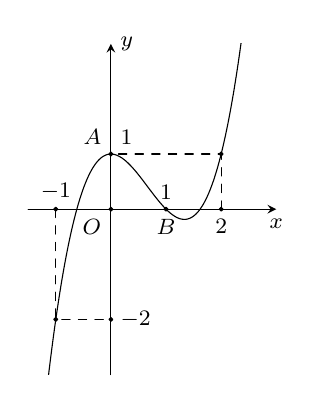
\begin{tikzpicture}[>=stealth,line join=round,line cap=round,font=\footnotesize,scale=0.7]
		\draw[->] (-1.5,0)--(3,0)node[below]{$x$};
		\draw[->] (0,-3)--(0,3)node[right]{$y$};
		\def\f(#1){(#1)^3-2*(#1)^2+1};
		\clip (-1.5,-3)rectangle (3,3);		
		\draw[smooth,samples=300]
		plot[domain=-1.5:3](\x,{\f(\x)});
		\draw[dashed] (-1,0)--(-1,-2)--(0,-2);
		\draw[dashed] (2,0)--(2,1)--(0,1);
		\draw[fill=black] (0,0) circle (1pt) node[below left]{$O$};
		\draw[fill=black] (-1,0) circle (1pt) node[above]{$-1$};
		\draw[fill=black] (2,0) circle (1pt) node[below]{$2$};
		\draw[fill=black] (1,0) circle (1pt) node[below]{$B$} node[above]{$1$};
		\draw[fill=black] (0,-2) circle (1pt) node[right]{$-2$};
		\draw[fill=black] (0,1) circle (1pt) node[above right]{$1$} node[above left]{$A$};
		\draw[fill=black] (-1,-2) circle (1pt);
		\draw[fill=black] (2,1) circle (1pt);
		\end{tikzpicture}
	}
	\loigiai{
		Ta có $g'(x)=f'(x)+2$.\\
		Cho $g'(x)=0\Leftrightarrow f'(x)=-2$.\\
		Dựa vào đồ thị ta thấy $f'(x)=-2\Leftrightarrow x=-1$.\\
		Bảng xét dấu của hàm số $g'(x)$ trên khoảng $(-\infty;0)$ như sau
		\begin{center}
			
\begin{tikzpicture}[>=stealth]
			\tkzTabInit[nocadre=false,lgt=1.2,espcl=2,deltacl=0.5]
			{$x$/.7 ,$g'(x)$/.7}
			{$-\infty$, $-1$, $0$}
			\tkzTabLine{,-,$0$,+,}
			\end{tikzpicture}
		\end{center}
		Vậy hàm số $g(x)$ đạt cực tiểu tại điểm $x=-1$.
	}
\end{ex}
\begin{ex}%[Dự án TLDH1-Nhóm Latex, Kiều Ngân]%[2D1B5-5]%Câu 3.
	\immini{
		Cho hàm số $y=f(x)$. Hàm số $y=f'(x)$ có đồ thị như hình vẽ. Khẳng định nào sau đây là khẳng định đúng?
		\choice
		{Đồ thị hàm số $y=f(x)$ có hai điểm cực trị}
		{Đồ thị hàm số $y=f(x)$ có một điểm cực trị}
		{\True Đồ thị hàm số $y=f(x)$ có ba điểm cực trị}
		{Đồ thị hàm số $y=f(x)$ cắt trục hoành tại ba điểm phân biệt}
	}{
		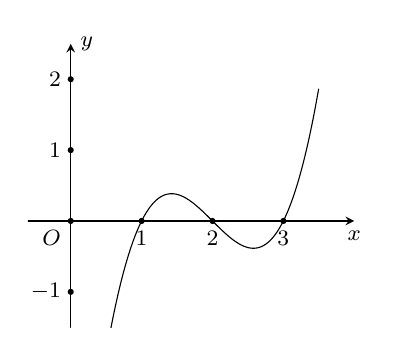
\begin{tikzpicture}[>=stealth,line join=round,line cap=round,font=\footnotesize,scale=0.9]
		\draw[->] (-0.6,0)--(4,0)node[below]{$x$};
		\draw[->] (0,-1.5)--(0,2.5)node[right]{$y$};
		\def\f(#1){(#1-1)*(#1-2)*(#1-3)};
		\clip (-0.6,-1.5)rectangle (4,2.5);		
		\draw[smooth,samples=300]
		plot[domain=0.5:3.5](\x,{\f(\x)});
		\draw[fill=black] (0,0) circle (1pt) node[below left]{$O$};
		\draw[fill=black] (3,0) circle (1pt) node[below]{$3$};
		\draw[fill=black] (2,0) circle (1pt) node[below]{$2$};
		\draw[fill=black] (1,0) circle (1pt) node[below]{$1$};
		\draw[fill=black] (0,-1) circle (1pt) node[left]{$-1$};
		\draw[fill=black] (0,1) circle (1pt) node[left]{$1$};
		\draw[fill=black] (0,2) circle (1pt) node[left]{$2$};
		\end{tikzpicture}
	}
	\loigiai{
		Ta có $f'(x)=0\Leftrightarrow\hoac{&x=1\\&x=2\\&x=3.}$ \\
		Phương trình có $3$ nghiệm đơn nên đồ thị hàm số $y=f(x)$ có ba điểm cực trị.}
\end{ex}
\begin{ex}%[Dự án TLDH1-Nhóm Latex, Kiều Ngân]%[2D1B5-5]%Câu 4.
	\immini{
		Gọi $(C)$ là đồ thị hàm số $y=f(x)$ như hình vẽ bên. Cho các mệnh đề sau:\\
		(I). $f'(-2)=1$;\\
		(II). $f'(0)=-2$;\\
		(III). $f'(2)=0$.\\
		Số mệnh đề đúng là 
		\choice
		{$1$}
		{\True $3$}
		{$0$}
		{$2$} 
	}{
		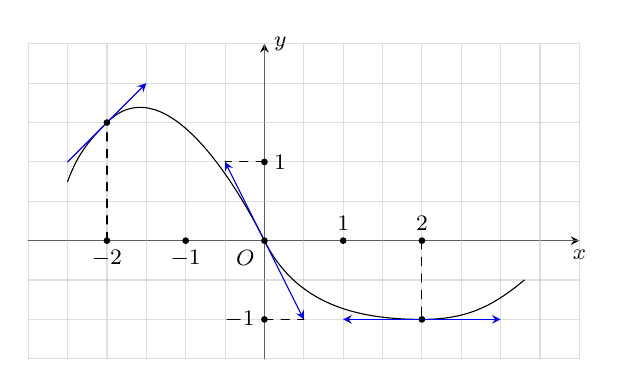
\begin{tikzpicture}[>=stealth,line join=round,line cap=round,font=\footnotesize,scale=1]
		\draw[->] (-3,0)--(4,0)node[below]{$x$};
		\draw[->] (0,-1.5)--(0,2.5)node[right]{$y$};
		\draw[gray!50,thin,opacity=.5]
		(-3,-1.5) grid (4,2.5);
		\draw[gray!50,thin,opacity=.5](-2.5,-1.5)--(-2.5,2.5) (-1.5,-1.5)--(-1.5,2.5) (-0.5,-1.5)--(-0.5,2.5) (0.5,-1.5)--(0.5,2.5) (1.5,-1.5)--(1.5,2.5) (2.5,-1.5)--(2.5,2.5) (3.5,-1.5)--(3.5,2.5);
		\draw[gray!50,thin,opacity=.5](-3,-1.5)--(4,-1.5) (-3,-0.5)--(4,-0.5) (-3,0.5)--(4,0.5) (-3,1.5)--(4,1.5) (-3,2.5)--(4,2.5);
		\draw (-2.5,0.75) to [out=70,in=225]
		(-2,1.5) to [out=45,in=116.57]
		(0,0) to [out=-63.43,in=180]
		(2,-1) to [out=0,in=-140]
		(3.3,-0.5);
		\draw [blue,->](-2.5,1)--(-1.5,2);
		\draw [blue,<->](-0.5,1)--(0.5,-1);
		\draw [blue,<->](1,-1)--(3,-1);
		\draw [dashed](-2,0)--(-2,1.5);
		\draw [dashed](2,0)--(2,-1);
		\draw [dashed](0,1)--(-0.5,1);
		\draw [dashed](0,-1)--(0.5,-1);
		\draw[fill=black] (0,0) circle (1pt) node[below left]{$O$};
		\draw[fill=black] (-2,0) circle (1pt) node[below]{$-2$};
		\draw[fill=black] (-1,0) circle (1pt) node[below]{$-1$};
		\draw[fill=black] (2,0) circle (1pt) node[above]{$2$};
		\draw[fill=black] (1,0) circle (1pt) node[above]{$1$};
		\draw[fill=black] (0,1) circle (1pt) node[right]{$1$};
		\draw[fill=black] (0,-1) circle (1pt) node[left]{$-1$};
		\draw[fill=black] (-2,1.5) circle (1pt);
		\draw[fill=black] (2,-1) circle (1pt);
		\end{tikzpicture}
	}
	\loigiai{
		Ta có $f'(x_0)$ là hệ số góc của phương trình tiếp tuyến với đồ thị hàm số $(C)$ tại điểm $x_0$.\\
		Dựa vào hình vẽ ta thấy số mệnh đề đúng là $3$.}
\end{ex}
\begin{ex}%[Dự án TLDH1-Nhóm Latex, Kiều Ngân]%[2D1K5-5]%Câu 5.
	\immini{
		Cho hàm số $y=f(x)$ có đồ thị $y=f'(x)$ cắt trục $Ox$ tại ba điểm có hoành độ $a<b<c$ như hình vẽ.
		Mệnh đề nào dưới đây là đúng?
		\choice
		{$f(c)>f(b)>f(a)$}
		{$f(a)>f(b)>f(c)$}
		{\True $f(c)+f(a)-2f(b)>0$}
		{$(f(b)-f(a))(f(b)-f(c))<0$}
	}{
		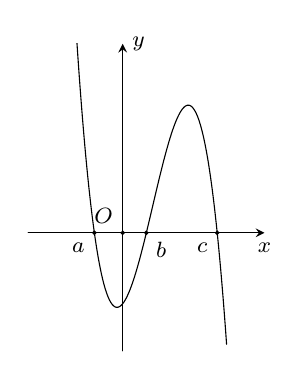
\begin{tikzpicture}[>=stealth,line join=round,line cap=round,font=\footnotesize,scale=0.6]
		\draw[->] (-2,0)--(3,0)node[below]{$x$};
		\draw[->] (0,-2.5)--(0,4)node[right]{$y$};
		\def\f(#1){-2.5*(#1+0.6)*(#1-0.5)*(#1-2)};
		\clip (-2,-2.5)rectangle (3,4);		
		\draw[smooth,samples=300]
		plot[domain=-1.1:2.2](\x,{\f(\x)});
		\draw[fill=black] (0,0) circle (1pt) node[above left]{$O$};
		\draw[fill=black] (-0.6,0) circle (1pt) node[below left]{$a$};
		\draw[fill=black] (0.5,0) circle (1pt) node[below right]{$b$};
		\draw[fill=black] (2,0) circle (1pt) node[below left]{$c$};
		\end{tikzpicture}
	}
	\loigiai{
		Dựa vào đồ thị ta có $f'(x)=0\Rightarrow\hoac{&x=a\\&x=b\\&x=c.}$\\
		Bảng biến thiên của hàm số $y=f(x)$ như sau 
		\begin{center}
			
\begin{tikzpicture}[>=stealth]
			\tkzTabInit[nocadre=false,lgt=1.2,espcl=2,deltacl=0.5]
			{$x$/.7 ,$f'(x)$/.7,$f(x)$/1.5}
			{$-\infty$, $a$, $b$, $c$, $+\infty$}
			\tkzTabLine{,+,$0$,-,$0$,+,$0$,-,}
			\tkzTabVar{-/,+/$f(a)$,-/$f(b)$,+/$f(c)$,-/}
			\end{tikzpicture}
		\end{center}
		Suy ra hàm số $y=f(x)$ có $3$ cực trị thỏa $f(a)>f(b)$, $f(c)>f(b)\Rightarrow f(c)+f(a)-2f(b)>0$.}
\end{ex}
\begin{ex}%[Dự án TLDH1-Nhóm Latex, Kiều Ngân]%[2D1G5-5]%Câu 6.
	\immini{
		Cho hàm số $y=f(x)$ có đạo hàm cấp một $f'(x)$ và đạo hàm cấp hai $f''(x)$ trên $\mathbb{R}$. Biết đồ thị của các hàm số $y=f(x)$, $y=f'(x)$, $y=f''(x)$ là một trong các đường cong $(C_1)$, $(C_2)$, $(C_3)$ như hình vẽ.
		Hỏi đồ thị của hàm số $y=f(x)$, $y=f'(x)$, $y=f''(x)$ lần lượt theo thứ tự nào dưới đây?
		\choice
		{$(C_2)$, $(C_1)$, $(C_3)$}
		{$(C_1)$, $(C_2)$, $(C_3)$}
		{\True $(C_3)$, $(C_2)$, $(C_1)$}
		{$(C_3)$, $(C_1)$, $(C_2)$}
	}{
		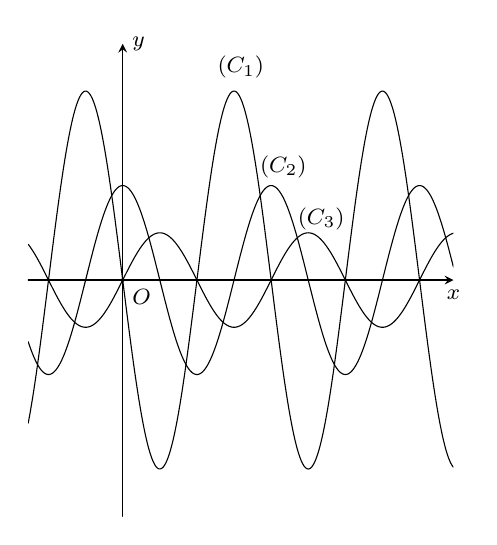
\begin{tikzpicture}[>=stealth,line join=round,line cap=round,font=\footnotesize,scale=0.6,x=0.5cm,y=1cm]
		\draw[->] (-4,0)--(14,0)node[below]{$x$};
		\draw[->] (0,-5)--(0,5)node[right]{$y$};
		\clip (-4,-5)rectangle (14,5);		
		\draw[smooth, samples=300]
		plot[domain=-4:14](\x,{sin(\x r)});
		\draw[smooth, samples=300]
		plot[x=0.5cm,y=2cm,domain=-4:14](\x,{cos(\x r)});
		\draw[smooth, samples=300]
		plot[x=0.5cm,y=4cm,domain=-4:14](\x,{-sin(\x r)});
		\draw[fill=black] (0,0) circle (1pt) node[below right]{$O$};
		\node at (5,4.5){$(C_1)$};
		\node at (6.8,2.4){$(C_2)$};
		\node at (8.4,1.3){$(C_3)$};
		\end{tikzpicture}
	}
	\loigiai{
		Ta nhận thấy đường $(C_1)$ và $(C_3)$ cùng cắt trục hoành tại cùng một điểm và hoành độ của điểm đó là cực trị của đường $(C_2)$. Và giao điểm của đường $(C_2)$ với trục hoành có hoành độ là hoành độ cực trị của hai đường còn lại.\\
		Ngoài ra, ta thấy phần đồ thị nằm dưới trục hoành của $(C_2)$ ứng với phần nghịch biến của $(C_3)$ và phần nằm trên trục hoành của $(C_2)$ ứng với phần đồng biến của $(C_3)$ nên đồ thị $(C_2)$ là đồ thị của hàm số $f'(x)$ là đạo hàm của hàm số có đồ thị $(C_3)$.\\
		Tương tự, phần đồ thị nằm dưới trục hoành của $(C_1)$ ứng với phần nghịch biến của $(C_2)$ và phần nằm trên trục hoành của $(C_1)$ ứng với phần đồng biến của $(C_2)$ nên đồ thị $(C_1)$ là đồ thị của hàm số $f''(x)$ là đạo hàm của hàm số có đồ thị $(C_2)$.}
\end{ex}
\begin{ex}%[Dự án TLDH1-Nhóm Latex, Kiều Ngân]%[2D1K5-5]%Câu 7.
	\immini{
		Cho hàm số $y=f(x)$ có đồ thị hàm số $y=f'(x)$ như hình vẽ. Xét hàm số $g(x)=2f(x)+2x^3-4x-3m-6\sqrt{5}$ với $m$ là số thực. Để $g(x)\leq 0,\forall x\in\left[-\sqrt{5};\sqrt{5}\right]$ thì điều kiện của $m$ là
		\choice
		{\True $m\geq\dfrac{2}{3}f(\sqrt{5})$}
		{$m\leq\dfrac{2}{3}f(\sqrt{5})$}
		{$m\leq\dfrac{2}{3}f(0)-2\sqrt{5}$}
		{$m\geq\dfrac{2}{3}f(-\sqrt{5})-4\sqrt{5}$}
	}{
		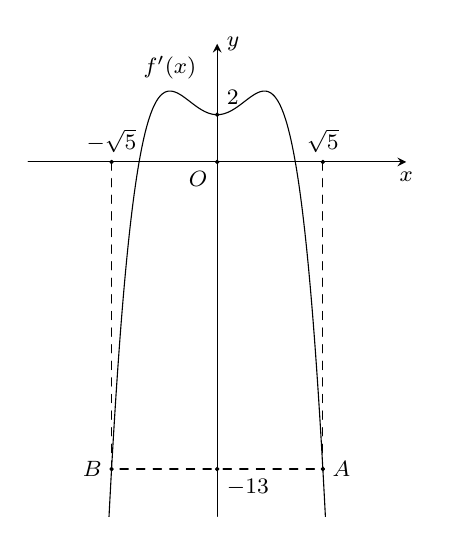
\begin{tikzpicture}[>=stealth,line join=round,line cap=round,font=\footnotesize,scale=0.6,x=1cm,y=0.5cm]
		\draw[->] (-4,0)--(4,0)node[below]{$x$};
		\draw[->] (0,-15)--(0,5)node[right]{$y$};
		\def\f(#1){-(#1)^4+2*(#1)^2+2};
		
		\clip (-4,-15) rectangle (4,5);		
		\draw[smooth, samples=300]
		plot[domain=-2.3:2.3](\x,{\f(\x)});
		\draw[fill=black] (0,0) circle (1pt) node[below left]{$O$};
		\draw[fill=black] (0,2) circle (1pt) node[above right]{$2$};
		\draw[fill=black] (-2.2361,0) circle (1pt) node[above]{$-\sqrt{5}$};
		\draw[fill=black] (2.2361,0) circle (1pt) node[above]{$\sqrt{5}$};
		\draw[fill=black] (0,-13) circle (1pt) node[below right]{$-13$};
		\draw[fill=black] (-2.2361,-13) circle (1pt) node[left]{$B$};
		\draw[fill=black] (2.2361,-13) circle (1pt) node[right]{$A$};
		\draw[dashed](-2.2361,0)--(-2.2361,-13)--(0,-13);
		\draw[dashed](2.2361,0)--(2.2361,-13)--(0,-13);
		\node at (-1,4){$f'(x)$};
		\end{tikzpicture}
	}
	\loigiai{
		\immini{
			Ta có
			\begin{eqnarray*}
				&&g(x)=2f(x)+2x^3-4x-3m-6\sqrt{5}\leq 0,\forall x\in\left[-\sqrt{5};\sqrt{5}\right]\\
				& \Leftrightarrow& 2f(x)+2x^3-4x-6\sqrt{5}\leq 3m,\forall x\in\left[-\sqrt{5};\sqrt{5}\right]\\
				& \Leftrightarrow& 3m\geq\max\limits_{\left[-\sqrt{5};\sqrt{5}\right]} h(x), \text{ với } h(x)=2f(x)+2x^3-4x-6\sqrt{5}.
			\end{eqnarray*}
			Xét hàm số $h(x)=2f(x)+2x^3-4x-6\sqrt{5}$.\\
			Ta có $h'(x)=2f'(x)+6x^2-4$;
			$h'(x)>0\Leftrightarrow f'(x)>2-3x^2$.\\ 
			Quan sát đồ thị hàm số $y=f'(x)$ và $y=2-3x^2$ trên cùng hệ trục tọa độ, có thể thấy $2$ đường cong có các điểm chung $(0;2)$, $(\sqrt{5};-13)$, $(-\sqrt{5};-13)$ và đồ thị hàm số $y=f'(x)$ luôn nằm trên đồ thị hàm số $y=2-3x^2$ nên $h'(x)\geq 0$ với mọi $x\in (-\sqrt{5},\sqrt{5})$ và trên khoảng đó $h'(x)$ chỉ bằng không tại điểm $x=0$, do đó $h'(x)$ đồng biến trên $\left[-\sqrt{5};\sqrt{5}\right]$.\\
			Suy ra $\max\limits_{x\in [-\sqrt{5};\sqrt{5}]} h(x)=h(\sqrt{5})=2f(\sqrt{5})$.\\
			Vậy điều kiện của $m$ là $m\geq\dfrac{2}{3}f(\sqrt{5})$.
		}{
			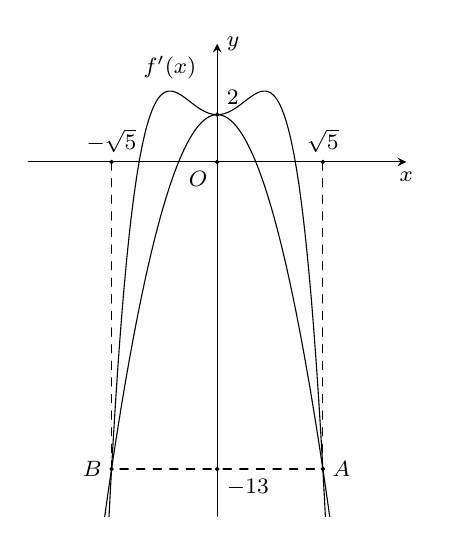
\begin{tikzpicture}[>=stealth,line join=round,line cap=round,font=\footnotesize,scale=0.6,x=1cm,y=0.5cm]
			\draw[->] (-4,0)--(4,0)node[below]{$x$};
			\draw[->] (0,-15)--(0,5)node[right]{$y$};
			\def\f(#1){-(#1)^4+2*(#1)^2+2};
			\def\g(#1){2-3*(#1)^2};
			
			\clip (-4,-15) rectangle (4,5);		
			\draw[smooth, samples=300]
			plot[domain=-2.3:2.3](\x,{\f(\x)});
			\draw[smooth, samples=300]
			plot[domain=-2.4:2.4](\x,{\g(\x)});
			\draw[fill=black] (0,0) circle (1pt) node[below left]{$O$};
			\draw[fill=black] (0,2) circle (1pt) node[above right]{$2$};
			\draw[fill=black] (-2.2361,0) circle (1pt) node[above]{$-\sqrt{5}$};
			\draw[fill=black] (2.2361,0) circle (1pt) node[above]{$\sqrt{5}$};
			\draw[fill=black] (0,-13) circle (1pt) node[below right]{$-13$};
			\draw[fill=black] (-2.2361,-13) circle (1pt) node[left]{$B$};
			\draw[fill=black] (2.2361,-13) circle (1pt) node[right]{$A$};
			\draw[dashed](-2.2361,0)--(-2.2361,-13)--(0,-13);
			\draw[dashed](2.2361,0)--(2.2361,-13)--(0,-13);
			\node at (-1,4){$f'(x)$};
			\end{tikzpicture}
		}
		}
\end{ex}
\begin{ex}%[Dự án TLDH1-Nhóm Latex, Kiều Ngân]%[2D1K5-5]%Câu 8.
	\immini{
		Cho hàm số $y=f(x)$. Hàm số $y=f'(x)$ có đồ thị như hình bên. Hàm số $f(x^2)$ đồng biến trên khoảng
		\choice
		{$(0;\sqrt{3})$}
		{\True $\left(-\sqrt{3};0\right)$}
		{$(0;+\infty)$}
		{$\left(-\infty;-\sqrt{3}\right)$}
	}{
		\begin{tikzpicture}[>=stealth,line join=round,line cap=round,font=\footnotesize,scale=0.6]
		\draw[->] (-3,0)--(4,0)node[below]{$x$};
		\draw[->] (0,-5)--(0,2)node[right]{$y$};
		\def\f(#1){0.7*(#1+2)*(#1-3)};
		\clip (-3,-7)rectangle (4,2);		
		\draw[smooth,samples=300]
		plot[domain=-2.2:3.2](\x,{\f(\x)});
		\draw[fill=black] (0,0) circle (1pt) node[below left]{$O$};
		\draw[fill=black] (-2,0) circle (1pt) node[below left]{$-2$};
		\draw[fill=black] (3,0) circle (1pt) node[below right]{$3$};
		\end{tikzpicture}
	}
	\loigiai{
		Ta có $y'=2xf'(x^2)$.\\
		Hàm số đồng biến $\Leftrightarrow y'>0\Leftrightarrow 2xf'(x^2)>0$\\
		$$\Leftrightarrow\hoac{&\heva{&x>0\\&f'(x^2)>0}\\&\heva{&x<0\\&f'(x^2)<0}}
		\Leftrightarrow\hoac{&\heva{&x>0\\&x^2>3}\\&\heva{&x<0\\&x^2<3}}\Leftrightarrow\hoac{&\heva{&x>0\\&\hoac{&x>\sqrt{3}\\&x <-\sqrt{3}}}\\&\heva{&x<0\\&-\sqrt{3}<x<\sqrt{3}}}\Leftrightarrow\hoac{&x>\sqrt{3}\\&-\sqrt{3}<x<0.}$$
		Vậy hàm số đồng biến trên các khoảng $\left(-\sqrt{3};0\right)$ và $\left(\sqrt{3};+\infty\right)$.}
\end{ex}
\begin{ex}%[Dự án TLDH1-Nhóm Latex, Kiều Ngân]%[2D1K5-5]%Câu 9.
	\immini{
		Cho hàm số $y=f(x)=\dfrac{ax+b}{cx+d}$ $\left(a, b, c, d\in\mathbb{R}; c\neq 0; d\neq 0\right)$ có đồ thị $(C)$. Đồ thị của hàm số $y=f'(x)$ như hình vẽ bên. Biết $(C)$ cắt trục tung tại điểm có tung độ bằng $2$. Tiếp tuyến của $(C)$ tại giao điểm của $(C)$ với trục hoành có phương trình là
		\choice
		{\True $x+3y-2=0$}
		{$x+3y+2=0$}
		{$x-3y-2=0$}
		{$x-3y+2=0$}
	}{
		\begin{tikzpicture}[>=stealth,line join=round,line cap=round,font=\footnotesize,scale=0.6]
		\draw[->] (-5,0)--(5,0)node[below]{$x$};
		\draw[->] (0,-4)--(0,2)node[right]{$y$};
		\def\f(#1){(-3)/(#1+1)^2};
		\def\g(#1){(-3)/(#1+1)^2};
		\clip (-5,-4)rectangle (5,2);		
		\draw[smooth,samples=300]
		plot[domain=-0.5:3.5](\x,{\f(\x)});
		\draw[smooth,samples=300]
		plot[domain=-5:-1.5](\x,{\g(\x)});
		\draw[fill=black] (0,0) circle (1pt) node[below left]{$O$};
		\draw[fill=black] (-2,0) circle (1pt) node[above]{$-2$};
		\draw[fill=black] (-1,0) circle (1pt) node[above]{$-1$};
		\draw[fill=black] (0,-3) circle (1pt) node[right]{$-3$};
		\draw[fill=black] (-2,-3) circle (1pt);
		\draw[fill=black] (0,-1) circle (1pt);
		\draw[fill=black] (0,-2) circle (1pt);
		\draw[dashed](-2,0)--(-2,-3)--(0,-3);
		\draw[dashed](-1,-4)--(-1,2);
		\node at (3.5,-0.8){$y=f'(x)$};
		\end{tikzpicture}
	}
	\loigiai{
		$(C)$ cắt trục tung tại điểm có tung độ bằng $2$ nên $2=\dfrac{b}{d}\Rightarrow b=2d \quad (1)$.\\
		Ta có $y'=\dfrac{ad-bc}{(cx+d)^2}$.\\
		Đồ thị hàm số $y=f'(x)$ đi qua các điểm $A(-2;-3)$ và $B(0;-3)$ nên $\heva{&-3=\dfrac{ad-bc}{(-2c+d)^2}\quad (2)\\&-3=\dfrac{ad-bc}{d^2}\quad(3).}$ \\
		Đồ thị của hàm số $y=f'(x)$ có tiệm cận đứng $x=-1\Rightarrow-c+d=0\Rightarrow c=d \quad (4)$.\\
		Thế $(1)$, $(4)$ vào $(2)$ và $(3)$ ta có $\heva{&-3=\dfrac{ad-2d\cdot d}{(-2d+d)^2}\\&-3=\dfrac{ad-2d\cdot d}{d^2}}\Rightarrow\heva{&-3=\dfrac{a-2d}{d}\\&-3=\dfrac{a-2d}{d}}\Rightarrow-d=a$.\\
		Với $y=0\Rightarrow\dfrac{ax+b}{cx+d}=0\Rightarrow x=-\dfrac{b}{a} =-\dfrac{2d}{-d} =2$.\\
		Với $x=2\Rightarrow y'(2)=\dfrac{ad-bc}{(2c+d)^2} =\dfrac{-d^2-2d^2}{(2d+d)^2} =-\dfrac{1}{3}$.\\
		Do đó tiếp tuyến của $(C)$ tại giao điểm của $(C)$ với trục hoành có phương trình là
		$$y=-\dfrac{1}{3}(x-2)\Leftrightarrow 3y=-x+2\Leftrightarrow x+3y-2=0.$$}
\end{ex}
\begin{ex}%[Dự án TLDH1-Nhóm Latex, Kiều Ngân]%[2D1K5-5]%Câu 10.
	\immini{
		Cho hàm số $y=f(x)$. Hàm số $y=f'(x)$ có đồ thị như hình bên. Hàm số $y=f(3-2x)$ nghịch biến trên khoảng
		\choice
		{$(-1;+\infty)$}
		{$(0;2)$}
		{\True $(-\infty;-1)$}
		{$(1;3)$}
	}{
		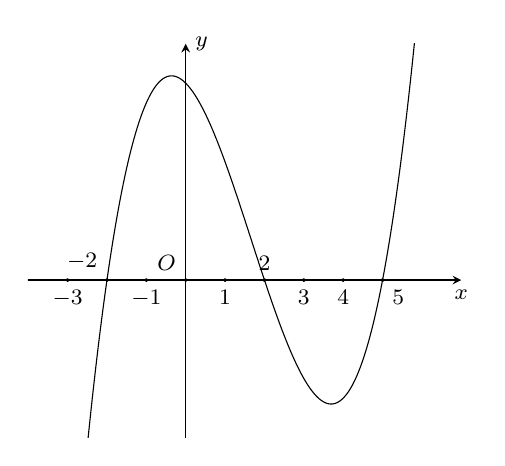
\begin{tikzpicture}[>=stealth,line join=round,line cap=round,font=\footnotesize,scale=0.5]
		\draw[->] (-4,0)--(7,0)node[below]{$x$};
		\draw[->] (0,-4)--(0,6)node[right]{$y$};
		\def\f(#1){0.25*(#1+2)*(#1-2)*(#1-5)};
		\clip (-4,-4)rectangle (7,6);		
		\draw[smooth,samples=300]
		plot[domain=-2.5:6.5](\x,{\f(\x)});
		\draw[fill=black] (0,0) circle (1pt) node[above left]{$O$};
		\draw[fill=black] (-3,0) circle (1pt) node[below]{$-3$};
		\draw[fill=black] (-2,0) circle (1pt) node[above left]{$-2$};
		\draw[fill=black] (-1,0) circle (1pt) node[below]{$-1$};
		\draw[fill=black] (1,0) circle (1pt) node[below]{$1$};
		\draw[fill=black] (2,0) circle (1pt) node[above]{$2$};
		\draw[fill=black] (3,0) circle (1pt) node[below]{$3$};
		\draw[fill=black] (4,0) circle (1pt) node[below]{$4$};
		\draw[fill=black] (5,0) circle (1pt) node[below right]{$5$};
		\end{tikzpicture}
	}
	\loigiai{		
		Ta có $y'=-2 f(3-2x)$.\\
		$y'<0\Leftrightarrow f(3-2x)>0\Leftrightarrow\hoac{&3-2x>5\\&-2<3-2x<2}\Leftrightarrow\hoac{&x <-1\\&\dfrac{1}{2}<x<\dfrac{5}{2}.}$ \\
		Vậy hàm số nghịch biến trên $(-\infty-1)$ và $\left(\dfrac{1}{2};\dfrac{5}{2}\right)$.}
\end{ex}
\begin{ex}%[Dự án TLDH1-Nhóm Latex, Kiều Ngân]%[2D1K5-5]%Câu 11.
	\immini{
		Cho hàm số $y=f(x)$ có đồ thị $y=f'(x)$ như hình vẽ (đồ thị $f'(x)$ cắt $Ox$ ở các điểm có hoành độ lần lượt là $1$, $2$, $5$, $6$). Chọn khẳng định đúng?
		\choice
		{$f(x)$ nghịch biến trên khoảng $(1;2)$}
		{\True $f(x)$ đồng biến trên khoảng $(5;6)$}
		{$f(x)$ nghịch biến trên khoảng $(1;5)$}
		{$f(x)$ đồng biến trên khoảng $(4;5)$}
	}{
		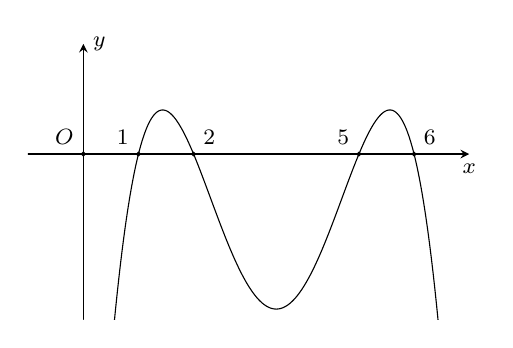
\begin{tikzpicture}[>=stealth,line join=round,line cap=round,font=\footnotesize,scale=0.7]
		\draw[->] (-1,0)--(7,0)node[below]{$x$};
		\draw[->] (0,-3)--(0,2)node[right]{$y$};
		\def\f(#1){-0.2*(#1-1)*(#1-2)*(#1-5)*(#1-6)};
		\clip (-1,-3)rectangle (7,2);		
		\draw[smooth,samples=300]
		plot[domain=0.5:6.5](\x,{\f(\x)});
		\draw[fill=black] (0,0) circle (1pt) node[above left]{$O$};
		\draw[fill=black] (1,0) circle (1pt) node[above left]{$1$};
		\draw[fill=black] (2,0) circle (1pt) node[above right]{$2$};
		\draw[fill=black] (5,0) circle (1pt) node[above left]{$5$};
		\draw[fill=black] (6,0) circle (1pt) node[above right]{$6$};
		\end{tikzpicture}
	}
	\loigiai{
		Bảng biến thiên
		\begin{center}
			
\begin{tikzpicture}[>=stealth]
			\tkzTabInit[nocadre=false,lgt=1.2,espcl=2,deltacl=0.5]
			{$x$/.7 ,$f'(x)$/.7,$f(x)$/1.5}
			{$-\infty$, $1$, $2$, $5$, $6$, $+\infty$}
			\tkzTabLine{,-,$0$,+,$0$,-,$0$,+,$0$,-}
			\tkzTabVar{+/,-/,+/,-/,+/,-/}
			\end{tikzpicture}
		\end{center}
		Dựa vào bảng biến thiên ta có $f(x)$ đồng biến trên khoảng $(5;6)$.}
\end{ex}
\begin{ex}%[Dự án TLDH1-Nhóm Latex, Kiều Ngân]%[2D1K5-5]%Câu 12.
	\immini{
		Cho hàm số $y=f(x)$ có đồ thị $y=f'(x)$ trên $\mathbb{R}$ như hình vẽ (trên $\mathbb{R}$ thì đồ thị $y=f'(x)$ là một nét liền và chỉ có $4$ điểm chung với $Ox$ tại các điểm có hoành độ lần lượt là $-1$; $1$; $2$; $4$). Đặt $g(x)=f(1-x)$. Chọn khẳng định đúng
		\choice
		{$g(x)$ đồng biến trên $(-3;0)$}
		{\True $g(x)$ đồng biến trên $(-4;-3)$}
		{$g(x)$ nghịch biến trên $(-1;0)$}
		{$g(x)$ đồng biến trên $(-4;-3)$ và $(0;2)$}
	}{
		\begin{tikzpicture}[>=stealth,line join=round,line cap=round,font=\footnotesize,scale=0.8]
		\draw[->] (-2,0)--(5,0)node[below]{$x$};
		\draw[->] (0,-1)--(0,3)node[right]{$y$};
		\def\f(#1){-0.25*(#1+1)*(#1-1)*(#1-2)*(#1-4)};
		\clip (-2,-1)rectangle (5,4);		
		\draw[smooth,samples=300]
		plot[domain=-1.2:4.5](\x,{\f(\x)});
		\draw[fill=black] (0,0) circle (1pt) node[below left]{$O$};
		\draw[fill=black] (1,0) circle (1pt) node[below]{$1$};
		\draw[fill=black] (2,0) circle (1pt) node[below]{$2$};
		\draw[fill=black] (4,0) circle (1pt) node[above left]{$4$};
		\draw[fill=black] (-1,0) circle (1pt) node[above left]{$-1$};
		\end{tikzpicture}
	}
	\loigiai{
		Ta có $g'(x)=f'(1-x)(1-x)'=-f'(1-x)$.\\
		 $g'(x)=0\Leftrightarrow\hoac{&1-x=-1\\&1-x=1\\&1-x=2\\&1-x=4}\Leftrightarrow\hoac{&x=2\\&x=0\\&x=-1\\&x=-3.}$ \\
		 $g'(x)>0\Leftrightarrow f'(1-x)<0\Leftrightarrow\hoac{&1-x<-1\\&1<1-x<2\\&1-x>4}\Leftrightarrow\hoac{&x>2\\&-1<x<0\\&x<-3.}$\\
		Bảng biến thiên của hàm số $g(x)$
		\begin{center}
			
\begin{tikzpicture}[>=stealth]
			\tkzTabInit[nocadre=false,lgt=1.2,espcl=2,deltacl=0.5]
			{$x$/.7 ,$g'(x)$/.7,$g(x)$/1.5}
			{$-\infty$, $-3$, $-1$, $0$, $2$, $+\infty$}
			\tkzTabLine{,+,$0$,-,$0$,+,$0$,-,$0$,+}
			\tkzTabVar{-/,+/,-/,+/,-/,+/}
			\end{tikzpicture}
		\end{center}
		Vậy $g(x)$ đồng biến trên $(-4;-3)$.}
\end{ex}
\begin{ex}%[Dự án TLDH1-Nhóm Latex, Kiều Ngân]%[2D1K5-5]%Câu 13.
	\immini{
		Cho hàm số $y=f(x)$ có đồ thị hàm $y=f'(x)$ như hình vẽ. Xét hàm số $g(x)=f(x)-\dfrac{1}{3}x^3-\dfrac{3}{4}x^2+\dfrac{3}{2}x+1$. Trong $4$ mệnh đề sau đây\\
		(I). $g(-3)<g(-1)$.\\
		(II). Hàm số $g(x)$ đồng biến trên $(-3;1)$.\\
		(III). $\min\limits_{x\in[-1;0]} g(x)=g(-1)$.\\
		(IV). $\max\limits_{x\in[-3;1]} g(x)=\max\{g(-3),g(1)\}$.\\
		Số mệnh đề đúng là 
		\choice
		{\True $2$}
		{$1$}
		{$3$}
		{$4$}
	}{
		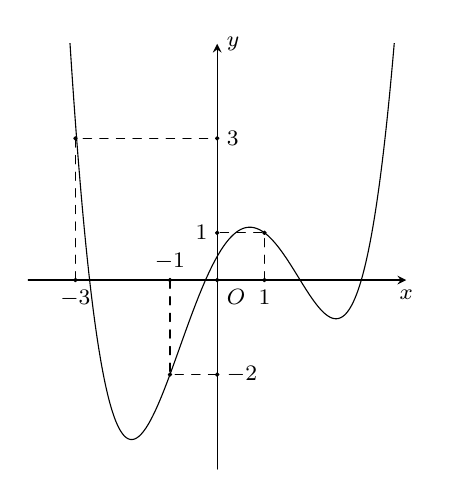
\begin{tikzpicture}[>=stealth,line join=round,line cap=round,font=\footnotesize,scale=0.6]
		\draw[->] (-4,0)--(4,0)node[below]{$x$};
		\draw[->] (0,-4)--(0,5)node[right]{$y$};
		\def\f(#1){0.14*(#1)^4-0.26*(#1)^3-1.14*(#1)^2+1.76*(#1)+0.5};
		\clip (-4,-4)rectangle (4,5);		
		\draw[smooth,samples=300]
		plot[domain=-3.2:3.9](\x,{\f(\x)});
		\draw[dashed] (-3,0)--(-3,3)--(0,3);
		\draw[dashed] (-1,0)--(-1,-2)--(0,-2);
		\draw[dashed] (1,0)--(1,1)--(0,1);
		\draw[fill=black] (0,0) circle (1pt) node[below right]{$O$};
		\draw[fill=black] (-3,0) circle (1pt) node[below]{$-3$};
		\draw[fill=black] (1,0) circle (1pt) node[below]{$1$};
		\draw[fill=black] (-1,0) circle (1pt) node[above]{$-1$};
		\draw[fill=black] (0,-2) circle (1pt) node[right]{$-2$};
		\draw[fill=black] (0,1) circle (1pt) node[left]{$1$};
		\draw[fill=black] (0,3) circle (1pt) node[right]{$3$};
		\draw[fill=black] (-1,-2) circle (1pt);
		\draw[fill=black] (-3,3) circle (1pt);
		\draw[fill=black] (1,1) circle (1pt);
		\end{tikzpicture}
	}
	\loigiai{
		\immini{
			Ta có $g'(x)=f'(x)-x^2-\dfrac{3}{2}x+\dfrac{3}{2} =f'(x)-\left(x^2+\dfrac{3}{2}x-\dfrac{3}{2}\right)$.\\
			Dựa vào đồ thị ta có $\heva{&f'(-1)=-2\\&f'(1)=1\\&f'(-3)=3}\Rightarrow\heva{&g'(-1)=0\\&g'(1)=0\\&g'(-3)=0.}$\\ 
			Vẽ parabol $(P)\colon y=x^2+\dfrac{3}{2}x-\dfrac{3}{2}$ trên cùng một hệ trục tọa độ với đồ thị hàm số $y=f'(x)$.\\
			Dựa vào đồ thị ta thấy:
			\begin{itemize}
				\item Trên khoảng $(-3;-1)$ thì $f'(x)<x^2+\dfrac{3}{2}x-\dfrac{3}{2}$ nên $g'(x)<0$, $\forall x\in(-3;-1)$.
				\item Trên khoảng $(-1;1)$ thì $f'(x)>x^2+\dfrac{3}{2}x-\dfrac{3}{2}$ nên $g'(x)>0$, $\forall x\in(-1;1)$.
			\end{itemize}
		}{
			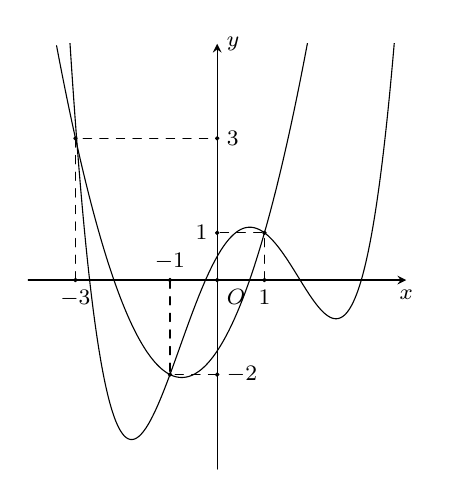
\begin{tikzpicture}[>=stealth,line join=round,line cap=round,font=\footnotesize,scale=0.6]
			\draw[->] (-4,0)--(4,0)node[below]{$x$};
			\draw[->] (0,-4)--(0,5)node[right]{$y$};
			\def\f(#1){0.14*(#1)^4-0.26*(#1)^3-1.14*(#1)^2+1.76*(#1)+0.5};
			\def\g(#1){(#1)^2+1.5*(#1)-1.5};
			\clip (-4,-4)rectangle (4,5);		
			\draw[smooth,samples=300]
			plot[domain=-3.2:3.9](\x,{\f(\x)});
			\draw[smooth,samples=300]
			plot[domain=-3.4:2.2](\x,{\g(\x)});
			\draw[dashed] (-3,0)--(-3,3)--(0,3);
			\draw[dashed] (-1,0)--(-1,-2)--(0,-2);
			\draw[dashed] (1,0)--(1,1)--(0,1);
			\draw[fill=black] (0,0) circle (1pt) node[below right]{$O$};
			\draw[fill=black] (-3,0) circle (1pt) node[below]{$-3$};
			\draw[fill=black] (1,0) circle (1pt) node[below]{$1$};
			\draw[fill=black] (-1,0) circle (1pt) node[above]{$-1$};
			\draw[fill=black] (0,-2) circle (1pt) node[right]{$-2$};
			\draw[fill=black] (0,1) circle (1pt) node[left]{$1$};
			\draw[fill=black] (0,3) circle (1pt) node[right]{$3$};
			\draw[fill=black] (-1,-2) circle (1pt);
			\draw[fill=black] (-3,3) circle (1pt);
			\draw[fill=black] (1,1) circle (1pt);
			\end{tikzpicture}
		}
		\noindent
		Do đó bảng biến thiên của hàm số $y=g(x)$ trên đoạn $[-3;1]$ như sau:\\
		\begin{center}
			
\begin{tikzpicture}[>=stealth]
			\tkzTabInit[nocadre=false,lgt=1.2,espcl=2.5,deltacl=0.8]
			{$x$/.7 ,$g'(x)$/.7,$g(x)$/2}
			{$-3$, $-1$, $1$}
			\tkzTabLine{$0$,-,$0$,+,$0$}
			\tkzTabVar{+/$g(-3)$,-/$g(-1)$,+/$g(1)$}
			\end{tikzpicture}
		\end{center}
		Từ bảng biến thiên suy ra:
		\begin{itemize}
			\item $g(-3)>g(-1)$: mệnh đề (I) sai.
			\item Hàm số $g(x)$ nghịch biến trên $(-3;-1)$ và đồng biến trên $(-1;1)$: mệnh đề (II) sai.
			\item $\min\limits_{x\in[-1;0]} g(x)=g(-1)$: mệnh đề (III) đúng.
			\item $\max\limits_{x\in[-3;1]} g(x)=\max\{g(-3),g(1)\}$: mệnh đề (IV) đúng.
		\end{itemize}
		Vậy số mệnh đề đúng là $2$.}
\end{ex}
\begin{ex}%[Dự án TLDH1-Nhóm Latex, Kiều Ngân]%[2D1K5-5]%Câu 14.
	\immini{
		Cho hàm số $y=f(x)$. Đồ thị của hàm số $y=f'(x)$ như hình vẽ bên. Đặt $M=\max\limits_{[-2; 6]} f(x)$, $m=\min\limits_{[-2; 6]} f(x)$, $T=M+m$. Mệnh đề nào dưới đây đúng?
		\choice
		{$T=f(0)+f(2)$}
		{\True $T=f(5)+f(-2)$}
		{$T=f(5)+f(6)$}
		{$T=f(0)+f(-2)$}
	}{
		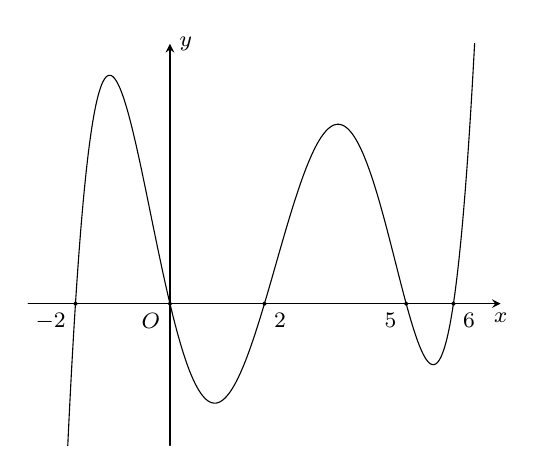
\begin{tikzpicture}[>=stealth,line join=round,line cap=round,font=\footnotesize,scale=0.6]
		\draw[->] (-3,0)--(7,0)node[below]{$x$};
		\draw[->] (0,-3)--(0,5.5)node[right]{$y$};
		\def\f(#1){0.035*(#1)*(#1+2)*(#1-2)*(#1-5)*(#1-6)};
		\clip (-3,-3)rectangle (7,5.5);		
		\draw[smooth,samples=300]
		plot[domain=-2.2:6.5](\x,{\f(\x)});
		\draw[fill=black] (0,0) circle (1pt) node[below left]{$O$};
		\draw[fill=black] (-2,0) circle (1pt) node[below left]{$-2$};
		\draw[fill=black] (2,0) circle (1pt) node[below right]{$2$};
		\draw[fill=black] (5,0) circle (1pt) node[below left]{$5$};
		\draw[fill=black] (6,0) circle (1pt) node[below right]{$6$};
		\end{tikzpicture}
	}
	\loigiai{
		Ta có $f'(x)=0\Leftrightarrow\hoac{&x=-2\\&x=0\\&x=2\\&x=5\\&x=6.}$ \\
		Bảng biến thiên
		\begin{center}
			
\begin{tikzpicture}[>=stealth]
			\tkzTabInit[nocadre=false,lgt=1.2,espcl=2,deltacl=0.7]
			{$x$/.7 ,$f'(x)$/.7,$f(x)$/2}
			{$-2$, $0$, $2$, $5$, $6$}
			\tkzTabLine{$0$,+,$0$,-,$0$,+,$0$,-,$0$}
			\tkzTabVar{-/$f(-2)$,+/$f(0)$,-/$f(2)$,+/$f(5)$,-/$f(6)$}
			\end{tikzpicture}
		\end{center}
		Từ đồ thị ta thấy
		\begin{itemize}
			\item $-\displaystyle\int\limits_0^2 f'(x)\mathrm{\,d}x<\displaystyle\int\limits_2^5 f'(x)\mathrm{\,d}x\Rightarrow-f(x)\bigg|_0^2<f(x)\bigg|_2^5\Rightarrow-f(2)+f(0)<f(5)-f(2)\Rightarrow f(0)<f(5)$\\
			$\Rightarrow M=f(5)$.
			\item $\displaystyle\int\limits_{-2}^{0} f'(x)\mathrm{\,d}x>-\displaystyle\int\limits_0^2 f'(x)\mathrm{\,d}x\Rightarrow f(x)\bigg|_{-2}^{0} >-f(x)\bigg|_0^2\Rightarrow f(0)-f(-2) >-f(2)+f(0)$\\
			$\Rightarrow f(-2)<f(2)$.
			\item $\displaystyle\int\limits_2^5 f'(x)\mathrm{\,d}x>-\displaystyle\int\limits_5^6 f'(x)\mathrm{\,d}x\Rightarrow f(x)\bigg|_2^5 >-f(x)\bigg|_5^6\Rightarrow f(5)-f(2) >-f(6)+f(5)\Rightarrow f(2)<f(6)$\\
			$\Rightarrow m=f(-2)$.
		\end{itemize}
		Vậy $T=f(5)+f(-2)$.}
\end{ex}
\begin{ex}%[Dự án TLDH1-Nhóm Latex, Kiều Ngân]%[2D1K5-5]%Câu 15.
	\immini{
		Đường cong trong hình vẽ bên là đồ thị hàm số $y=f'(x)$. Số điểm cực trị của hàm số $y=f(x)$ là
		\choice
		{$4$}
		{$3$}
		{$5$}
		{\True $2$}
	}{
		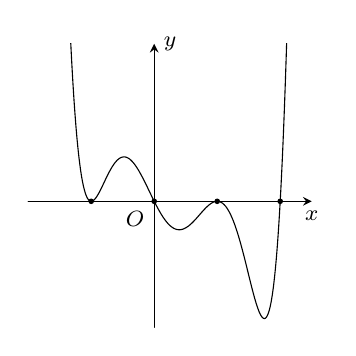
\begin{tikzpicture}[>=stealth,line join=round,line cap=round,font=\footnotesize,scale=0.8]
		\draw[->] (-2,0)--(2.5,0)node[below]{$x$};
		\draw[->] (0,-2)--(0,2.5)node[right]{$y$};
		\def\f(#1){1*(#1)*(#1+1)^2*(#1-1)^2*(#1-2)};
		\clip (-2,-2)rectangle (2.5,2.5);		
		\draw[smooth,samples=300]
		plot[domain=-1.5:2.5](\x,{\f(\x)});
		\draw[fill=black] (0,0) circle (1pt) node[below left]{$O$};
		\draw[fill=black] (-1,0) circle (1pt);
		\draw[fill=black] (1,0) circle (1pt);
		\draw[fill=black] (2,0) circle (1pt);
		\end{tikzpicture}
	}
	\loigiai{
		Gọi bốn nghiệm của phương trình $f'(x)=0$ lần lượt là $x_1<x_2<x_3<x_4$.\\
		Dựa vào đồ thị hàm số $y=f'(x)$ ta có bảng biến thiên của hàm số $y=f(x)$ như sau
		\begin{center}
			
\begin{tikzpicture}[>=stealth]
			\tkzTabInit[nocadre=false,lgt=1.2,espcl=2,deltacl=0.3]
			{$x$/.7 ,$f'(x)$/.7,$f(x)$/1.5}
			{,$x_1$, $x_2$, $x_3$, $x_4$,}
			\tkzTabLine{,+,$0$,+,$0$,-,$0$,-,$0$,+,}
			\tkzTabVar{-/,R,+/,R,-/,+/}
			\end{tikzpicture}
		\end{center}
		Dựa vào bảng biến thiên ta thấy hàm số $y=f(x)$ đạt cực trị tại $x_2$, $x_4$.}
\end{ex}
\begin{ex}%[Dự án TLDH1-Nhóm Latex, Kiều Ngân]%[2D1K5-5]%Câu 16.
	\immini{
		Cho hàm số $y=f(x)$ có đạo hàm là hàm $f'(x)$. Đồ thị của hàm số $y=f'(x)$ được cho như hình vẽ. Biết rằng $f(0)+f(3)=f(2)+f(5)$. Giá trị nhỏ nhất, giá trị lớn nhất của $y=f(x)$ trên đoạn $[0;5]$ lần lượt là
		\choice
		{\True $f(2)$; $f(5)$}
		{$f(0)$; $f(5)$}
		{$f(2)$; $f(0)$}
		{$f(1)$; $f(5)$}
	}{
		\begin{tikzpicture}[>=stealth,line join=round,line cap=round,font=\footnotesize,scale=0.7]
		\draw[->] (-1,0)--(6,0)node[below]{$x$};
		\draw[->] (0,-1.5)--(0,3)node[right]{$y$};	
		\clip (-1,-2)rectangle (6,3);
		\draw (-0.3,0.5) to [out=-60,in=120]
		(0,0) to [out=-60,in=175]
		(1,-0.9) to [out=5,in=230]
		(2,0) to [out=50,in=190]
		(5,2);	
		\draw[fill=black] (0,0) circle (1pt) node[below left]{$O$};
		\draw[fill=black] (5,0) circle (1pt) node[below]{$5$};
		\draw[dashed] (5,0)--(5,2);
		\draw[fill=black] (2,0) circle (1pt) node[below]{$2$};
		\node at (5,2.3){$y=f'(x)$};
		\end{tikzpicture}
	}
	\loigiai{
		Dựa vào đồ thị hàm số $f'(x)$ ta có bảng biến thiên
		\begin{center}
			
\begin{tikzpicture}[>=stealth]
			\tkzTabInit[nocadre=false,lgt=1.2,espcl=2.5,deltacl=0.8]
			{$x$/.7 ,$f'(x)$/.7,$f(x)$/2}
			{$0$, $2$, $5$}
			\tkzTabLine{$0$,-,$0$,+,}
			\tkzTabVar{+/$f(0)$,-/$f(2)$,+/$f(5)$}
			\end{tikzpicture}
		\end{center}
		Khi đó $\heva{&\min \limits_{[0;5]}f(x)=f(2)\\&f(3)>f(2).}$\\
		Mà $f(0)+f(3)=f(2)+f(5)\Rightarrow f(0)+f(2)<f(2)+f(5)\Rightarrow f(0)<f(5)$.\\
		Vậy giá trị nhỏ nhất, giá trị lớn nhất của $y=f(x)$ trên đoạn $[0;5]$ lần lượt là $f(2)$; $f(5)$.}
\end{ex}
\begin{ex}%[Dự án TLDH1-Nhóm Latex, Kiều Ngân]%[2D1K5-5]%Câu 17.
	\immini{
		Cho hàm số $y=f(x)$. Hàm số $y=f'(x)$ có đồ thị trên một khoảng $K$ như hình vẽ bên. Trong các khẳng định sau, có tất cả bao nhiêu khẳng định đúng?\\
		(I). Trên $K$, hàm số $y=f(x)$ có hai điểm cực trị.\\
		(II). Hàm số $y=f(x)$ đạt cực đại tại $x_3$.\\
		(III). Hàm số $y=f(x)$ đạt cực tiểu tại $x_1$.
		\choice
		{\True $2$}
		{$0$}
		{$1$}
		{$3$}
	}{
		\begin{tikzpicture}[>=stealth,line join=round,line cap=round,font=\footnotesize,scale=0.7]
		\draw[->] (-3,0)--(5,0)node[below]{$x$};
		\draw[->] (0,-3)--(0,5)node[right]{$y$};
		\def\f(#1){-0.1*(#1+1.9)*(#1-1)*(#1-3.6)^2};
		\clip (-3,-3)rectangle (5,5);		
		\draw[smooth,samples=300]
		plot[domain=-2.5:5](\x,{\f(\x)});
		\draw[fill=black] (0,0) circle (1pt) node[below left]{$O$};
		\draw[fill=black] (-1.9,0) circle (1pt) node[below left]{$x_1$};
		\draw[fill=black] (1,0) circle (1pt) node[above right]{$x_2$};
		\draw[fill=black] (3.6,0) circle (1pt) node[above]{$x_3$};
		\end{tikzpicture}
	}
	\loigiai{
		Bảng biến thiên của hàm số $y=f(x)$ như sau
		\begin{center}
			
\begin{tikzpicture}[>=stealth]
			\tkzTabInit[nocadre=false,lgt=1.2,espcl=2,deltacl=0.3]
			{$x$/.7 ,$f'(x)$/.7,$f(x)$/1.5}
			{,$x_1$, $x_2$, $x_3$,}
			\tkzTabLine{,-,$0$,+,$0$,-,$0$,-,}
			\tkzTabVar{+/,-/,+/,R,-/}
			\end{tikzpicture}
		\end{center}
		Theo bảng biến thiên, câu (I) và (III) là mệnh đề đúng.}
\end{ex}
\begin{ex}%[Dự án TLDH1-Nhóm Latex, Kiều Ngân]%[2D1K5-5]%Câu 18.
	\immini{
		Cho hàm số $y=f(x)$. Biết hàm số $y=f'(x)$ có đồ thị như hình vẽ bên.
		Hàm số $y=f\left(2x-3x^2\right)$ đồng biến trên khoảng nào dưới đây?
		\choice
		{$\left(\dfrac{1}{3};\dfrac{1}{2}\right)$}
		{$\left(\dfrac{1}{2};+\infty\right)$}
		{\True $\left(-\infty;\dfrac{1}{3}\right)$}
		{$\left(-2;\dfrac{1}{2}\right)$}
	}{
		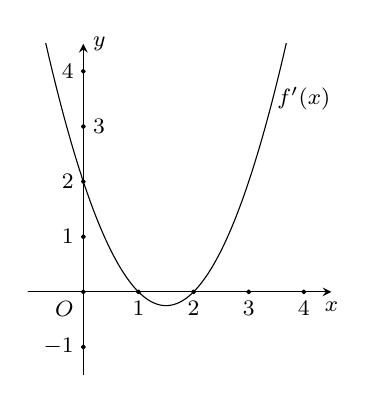
\begin{tikzpicture}[>=stealth,line join=round,line cap=round,font=\footnotesize,scale=0.7]
		\draw[->] (-1,0)--(4.5,0)node[below]{$x$};
		\draw[->] (0,-1.5)--(0,4.5)node[right]{$y$};
		\def\f(#1){(#1-1)*(#1-2)};
		\clip (-1,-1.5)rectangle (4.5,4.5);		
		\draw[smooth,samples=300]
		plot[domain=-0.7:3.7](\x,{\f(\x)});
		\draw[fill=black] (0,0) circle (1pt) node[below left]{$O$};
		\draw[fill=black] (1,0) circle (1pt) node[below]{$1$};
		\draw[fill=black] (2,0) circle (1pt) node[below]{$2$};
		\draw[fill=black] (4,0) circle (1pt) node[below]{$4$};
		\draw[fill=black] (0,1) circle (1pt) node[left]{$1$};
		\draw[fill=black] (0,2) circle (1pt) node[left]{$2$};
		\draw[fill=black] (0,3) circle (1pt) node[right]{$3$};
		\draw[fill=black] (0,4) circle (1pt) node[left]{$4$};
		\draw[fill=black] (0,-1) circle (1pt) node[left]{$-1$};
		\draw[fill=black] (3,0) circle (1pt) node[below]{$3$};
		\node at (4,3.5){$f'(x)$};
		\end{tikzpicture}
	}
	\loigiai{
		Đặt $u(x)=2x-3x^2 =\dfrac{1}{3}-3\left(x-\dfrac{1}{3}\right)^2\leq\dfrac{1}{3},\,\forall x\Rightarrow f'(u)>0,\,\forall u$.\\
		Ta có $f\left(2x-3x^2\right)=f\left(u(x)\right)$
		$ \Rightarrow\left[f\left(2x-3x^2\right)\right]'=f'(u)\cdot u'(x) =(2-6x)f'(u) $.\\
		Vì $f'(u)>0,\,\forall x$ nên $\left[f\left(2x-3x^2\right)\right]'>0\Leftrightarrow 2-6x>0\Leftrightarrow x<\dfrac{1}{3}$.}
\end{ex}
\begin{ex}%[Dự án TLDH1-Nhóm Latex, Kiều Ngân]%[2D1K5-5]%Câu 19.
	\immini{
		Cho hàm số $y=f(x)$ có đạo hàm liên tục trên $\mathbb{R}$. Đồ thị hàm số $y=f'(x)$ như hình vẽ bên. Số điểm cực trị của hàm số $g(x)=f(x)-4x$ là 
		\choice
		{$2$}
		{$3$}
		{\True $1$}
		{$4$}
	}{
		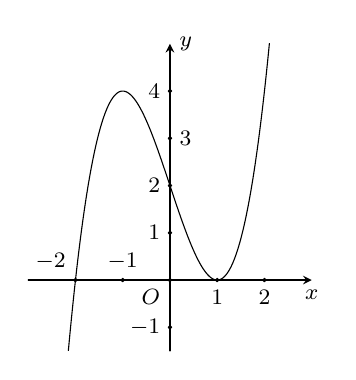
\begin{tikzpicture}[>=stealth,line join=round,line cap=round,font=\footnotesize,scale=0.6]
		\draw[->] (-3,0)--(3,0)node[below]{$x$};
		\draw[->] (0,-1.5)--(0,5)node[right]{$y$};
		\def\f(#1){(#1+2)*(#1-1)^2};
		\clip (-3,-1.5)rectangle (3,5);		
		\draw[smooth,samples=300]
		plot[domain=-2.2:2.2](\x,{\f(\x)});
		\draw[fill=black] (0,0) circle (1pt) node[below left]{$O$};
		\draw[fill=black] (1,0) circle (1pt) node[below]{$1$};
		\draw[fill=black] (2,0) circle (1pt)
		 node[below]{$2$};
		\draw[fill=black] (-1,0) circle (1pt) node[above]{$-1$};
		\draw[fill=black] (-2,0) circle (1pt) node[above left]{$-2$};
		\draw[fill=black] (4,0) circle (1pt) node[below]{$4$};
		\draw[fill=black] (0,1) circle (1pt) node[left]{$1$};
		\draw[fill=black] (0,2) circle (1pt) node[left]{$2$};
		\draw[fill=black] (0,3) circle (1pt) node[right]{$3$};
		\draw[fill=black] (0,4) circle (1pt) node[left]{$4$};
		\draw[fill=black] (0,-1) circle (1pt) node[left]{$-1$};
		\end{tikzpicture}
	}
	\loigiai{
		Ta có $g'(x)=f'(x)-4 =0\Leftrightarrow\hoac{&x=-1\\&x=2.}$ \\
		Bảng xét dấu $g(x)$ như sau
		\begin{center}
			
\begin{tikzpicture}[>=stealth]
			\tkzTabInit[nocadre=false,lgt=1.2,espcl=2,deltacl=0.6]
			{$x$/.7 ,$g'(x)$/.7}
			{$-\infty$, $-1$, $2$,$+\infty$}
			\tkzTabLine{,-,$0$,-,$0$,+,}
			\end{tikzpicture}
		\end{center}
		Vậy hàm số $g(x)$ có $1$ điểm cực trị.}
\end{ex}
\begin{ex}%[Dự án TLDH1-Nhóm Latex, Kiều Ngân]%[2D1K5-5]%Câu 20.
	\immini{
		Cho hàm số $y=f(x)$. Hàm số $y=f'(x)$ có đồ thị như hình bên. Hàm số $g(x)=f\left(x^2-1\right)$ đồng biến trên khoảng nào dưới đây?
		\choice
		{$(1;+\infty)$}
		{$(1;2)$}
		{\True $(0;1)$}
		{$(-2;-1)$}
	}{
		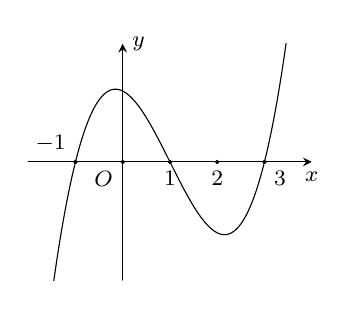
\begin{tikzpicture}[>=stealth,line join=round,line cap=round,font=\footnotesize,scale=0.6]
		\draw[->] (-2,0)--(4,0)node[below]{$x$};
		\draw[->] (0,-2.5)--(0,2.5)node[right]{$y$};
		\def\f(#1){0.5*(#1+1)*(#1-1)*(#1-3)};
		\clip (-2,-2.5)rectangle (4,2.5);		
		\draw[smooth,samples=300]
		plot[domain=-1.5:3.5](\x,{\f(\x)});
		\draw[fill=black] (0,0) circle (1pt) node[below left]{$O$};
		\draw[fill=black] (1,0) circle (1pt) node[below]{$1$};
		\draw[fill=black] (2,0) circle (1pt)
		node[below]{$2$};
		\draw[fill=black] (-1,0) circle (1pt) node[above left]{$-1$};
		\draw[fill=black] (3,0) circle (1pt) node[below right]{$3$};
		\end{tikzpicture}
	}
	\loigiai{
		\textbf{Cách 1:}\\ Ta có 
		$g'(x)=\left(f\left(x^2-1\right)\right)'=2xf'\left(x^2-1\right)$.\\
		Hàm số $g(x)$ đồng biến trên $(a;b)$ khi và chỉ khi $g'(x)\geq 0,\forall x\in(a;b)$.
		\begin{itemize}
			\item TH1: $\heva{&x\geq 0\\&-1\leq x^2-1\leq 1}\Leftrightarrow\heva{&x\geq 0\\&-\sqrt{2}\leq x\leq\sqrt{2}}\Leftrightarrow x\in[0;\sqrt{2}]$ mà $(0;1)\subset[0;\sqrt{2}]$.
			\item TH2: $\heva{&x\leq 0\\&1\leq x^2-1\leq 3}\Leftrightarrow x\in\left[-2;-\sqrt{2}\right]$.
			\item TH3: $\heva{&x\geq 0\\&x^2-1\geq 3}\Leftrightarrow\heva{&x\geq 0\\&\hoac{&x\leq-2\\&x\geq 2}}\Leftrightarrow x\geq 2$.
			\item TH4: $\heva{&x\leq 0\\&x^2-1 <-1}\Leftrightarrow\heva{&x\leq 0\\&x^2<0.}\Leftrightarrow x\in \varnothing$.
		\end{itemize}
		\textbf{Cách 2:}\\
		Ta có $f'(x)=(x+1)(x-1)(x-3)$.\\
		Do đó $g'(x)=2xf'\left(x^2-1\right)=2x^3\left(x^2-2\right)\left(x^2-4\right)$.\\
		Khi đó $g'(x)\geq 0\Leftrightarrow x\in\left[-2;-\sqrt{2}\right]\cup[0;\sqrt{2}]\cup[2;+\infty)$.\\
		Suy ra hàm số $y=g(x)$ đồng biến trên $(0;1)$.}
\end{ex}

\Closesolutionfile{ans}	

